\documentclass{standalone}
\usepackage{pgfplots}
\pgfplotsset{compat=1.18}

\begin{document}
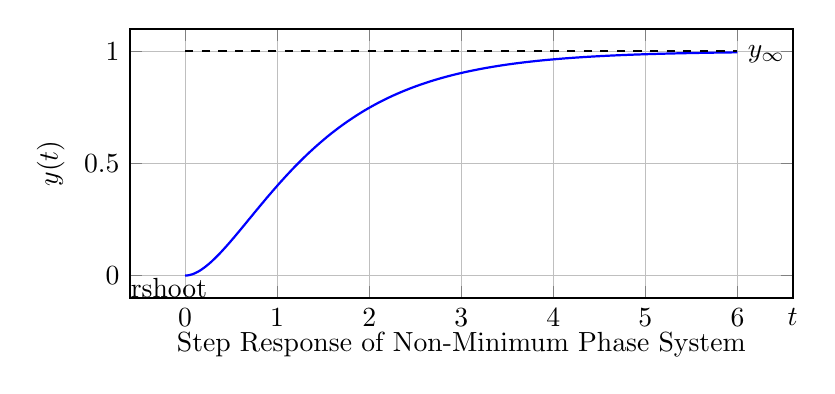
\begin{tikzpicture}
\begin{axis}[
  width=10cm,
  height=5cm,
  xlabel={$t$},
  ylabel={$y(t)$},
  grid=both,
  domain=0:6,
  samples=300,
  thick,
  title={Step Response of Non-Minimum Phase System},
  title style={at={(0.5,-0.15)}, anchor=north},
  xlabel style={at={(axis description cs:1,0)}, anchor=north},
]
  % Step response: y(t) = 1 - 2*exp(-t) + exp(-2t)
  \addplot[blue, thick] {1 - 2*exp(-x) + exp(-2*x)};
  
  % Steady-state line
  \addplot[dashed] coordinates {(0,1) (6,1)} node[right] {$y_\infty = 1$};
  
  % Annotate the initial undershoot
  \node[pin=150:{Initial undershoot}] at (axis cs:0.8,-0.25) {};
\end{axis}
\end{tikzpicture}
\end{document}
